\documentclass[../Master.tex]{subfiles}
% \bibliography{../Bibliography}

\begin{document}

\chapter{Result and discussion}

\section{Pyrazole Ligand Development}\label{sec:pyr-dev}

\subsection{Starting Materials}\label{sec:starting-materials}

While several ligands were synthesized and utilized within the research group led by Professor L. Carlucci, my specific contribution focused exclusively on one of these ligands, that is based upon an already studied one. The structure of the starting material, 4,4’-malonyldibenzoic, and the retrosynthetic approch to it is reported.

\begin{figure}[h]
	\centering
	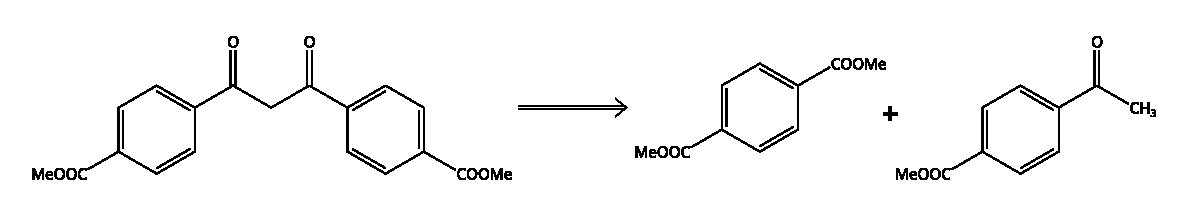
\includegraphics[width=16cm,height=8cm,keepaspectratio]{Structures/dikest2-retro.eps}
	\caption{4,4’-malonyldibenzoic acid Retrosynthesis Approach}\label{fig:dikest2-retro}
\end{figure}

The synthesis of the ligand is based on the cross-Claisen condensation followed by the hydrolisis of methylesters groups. The reaction was conducted with excellent yields and purity, resulting in the production of tens of grams of the compound. The reagents required for the synthesis are readily available commercially, facilitating the accessibility and reproducibility of the process. \\
The same synthetic approach has been carried out over a wide range of analogue compound, resulting tipically in high yield scalable reaction, as an example the ligand that will be analyzed in the section\ \ref{sec:electrochemistry} has been approached with the same strategies.\\
The detailed information on the synthesis and charactherization of 4,4’-malonyldibenzoic are reported in the section\ \ref{cha:experimental-section}.
\newpage
\subsection{Pyrazole Ligand Retrosynthesis}\label{sec:pyrazole-reaction}
Starting from the 1,3-diketone diester intermediate, obtained from the cross Claisen condensation, the apparently easier way to procede with the pyrazole formation is using hydrazine, of which a brief reaction mechanism is reported.

\begin{figure}[h!]
	\centering
	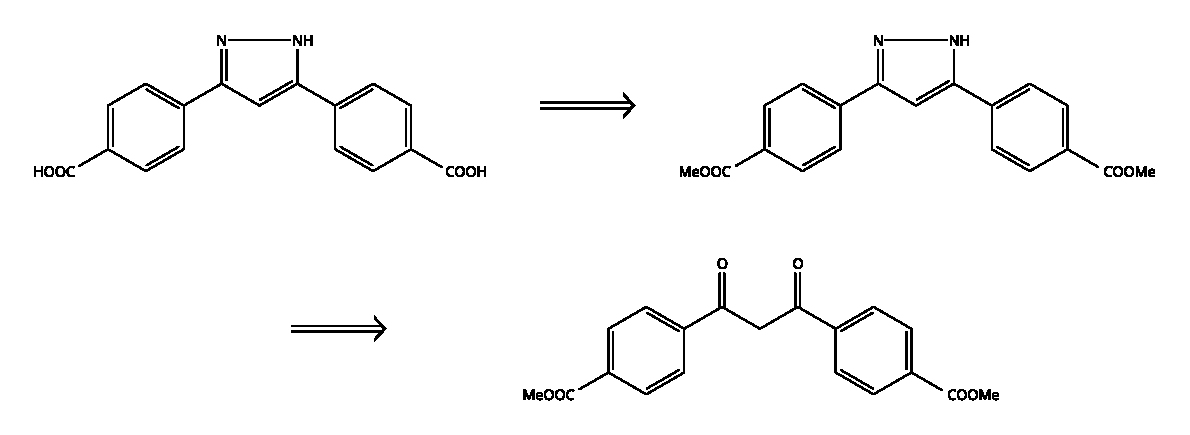
\includegraphics[width=16cm,height=8cm,keepaspectratio]{Structures/pyrazole-retro.eps}
	\caption{Pyrazole Ligand Retrosynthesis}\label{fig:pyrazole-retro}
\end{figure}

Typically the reaction reaches completion in ethanol under reflux conditions with an excess of hydrazine within a few hours withouth any catalyzer: in this specific case several problems has been encountered and analyzed.\\

\begin{figure}[h!]
	\centering
	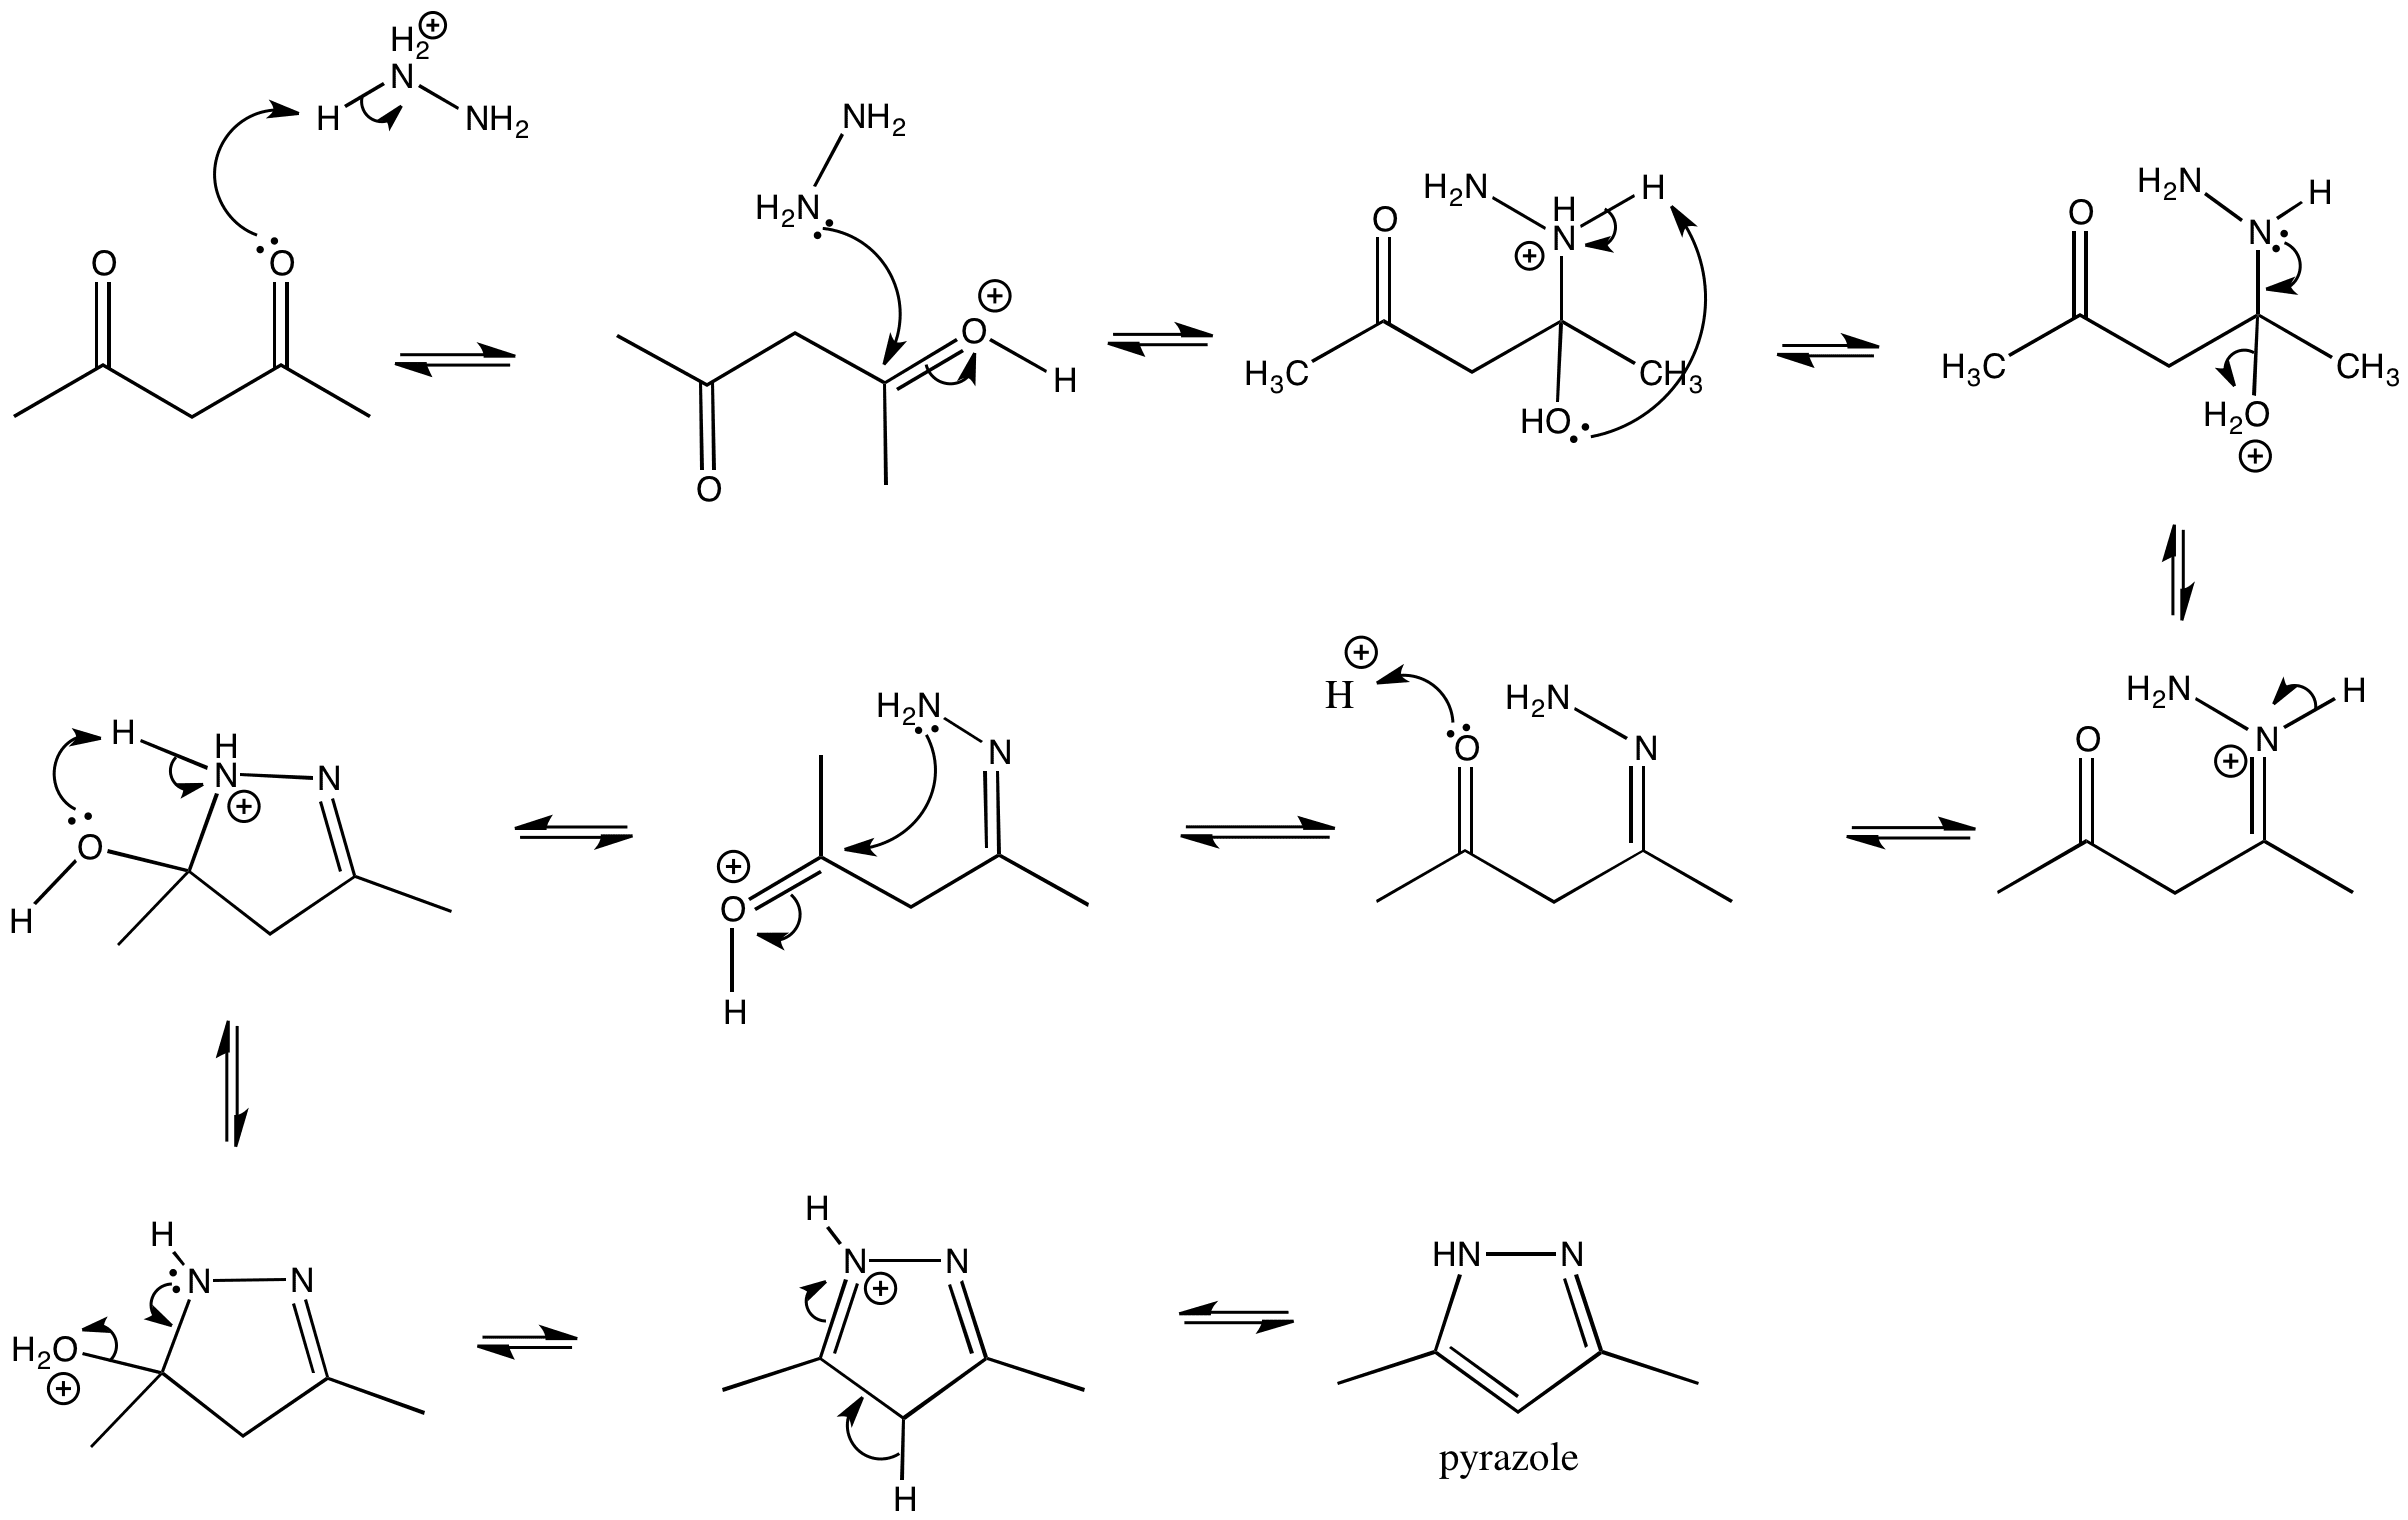
\includegraphics[width=16cm,height=8cm,keepaspectratio]{Images/pyrazole-mechanism.png}
	\caption{Pyrazole Formation Mechanism}
\end{figure}
\newline
After hydrazine addition the diester intermediate must undergo hydrolisis to obtain the corrisponding dibenzoic acid. The conditions for this step have also been analyzed.

\subsection{Pyrazole Diester Formation}\label{sec:pyrazole-diester}

During the iterative process of analysing the reaction condition, certain key characteristics of the starting reagent and the product of interest were crucial. The diketone intermediate possesses a characteristic straw-yellow colour, and also exhibits photoluminescence in the yellow-green range easily observed with a UV lamp. The pyrazole product is whitish in colour and returns intense blue emission.\\
Numerous variables influencing the course of the reaction were evaluated, the results of which are given below. The use of IR spectroscopy and NMR structural analysis was instrumental in recognising the products formed and also the mixtures left over from failed reactions, especially in the first attempts.

\begin{figure}[h!]
	\centering
	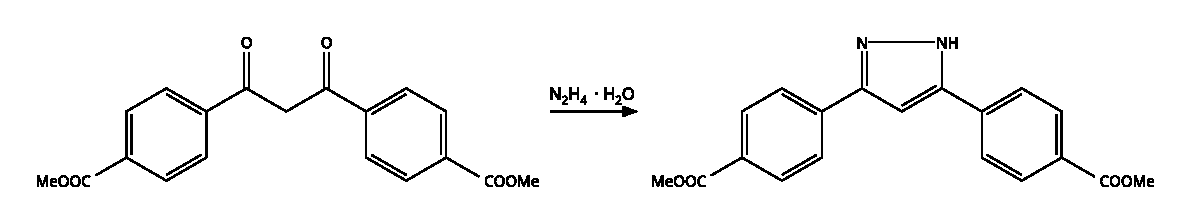
\includegraphics[width=13cm,height=8cm,keepaspectratio]{Structures/pyrazole-form.eps}
	\caption{Pyrazole Formation}\label{fig:pyrazole-form}
\end{figure}

\subsubsection{Solvent Choice and Reagent Solubility}\label{sec:solvent}

Dimethyl 4,4’-malonyldibenzoate is poorly soluble in most organic solvents, even after careful grinding and sonication. Different alternatives has been evaluated, noting that the solvent choice was highly restricted from the fact that 65\% hydrazine in water has been initially used. \\
Given the relatively low polarity of the ester functionalities, it would be beneficial to use a less polar solvent that still allows for the formation of a single phase with hydrazine water solution, while avoiding reactions with it.\\
The so low solubility can be attributed to several characteristic of the compound that is an highly simmetric diester. The correlation between solubility and symmetry of a molecule can vary depending on various factors, including the specific nature of the molecule and the solvent in which it is dissolved. While symmetry can influence certain aspects of a molecule's behavior, such as its physical properties, there is no general rule or direct correlation between solubility and symmetry. For example, symmetric molecules may have a more compact shape, which could reduce the surface area available for interaction with the solvent molecules. This can potentially lead to lower solubility if the solvent relies on surface interactions for dissolution. On the other hand, highly symmetrical molecules may have fewer polar or charged groups, which can reduce their ability to form favorable interactions with polar solvents. Other factors, such as temperature, pressure, and the presence of specific functional groups, can also significantly impact solubility. Experimental data and detailed analysis of the specific compound of interest are often required to accurately determine its solubility characteristics.

For these reasons the use of different solvent has been investigated, involving different approch for product recovery subsequently to solvent properties. \\
Reaction conducted in EtOH gives below 30\% yield and overnight reaction time is needed to observe appreciable product formation. Nevertheless the solvent was easily removable by evaporation and the product can be easily purified afterward.\\
The use of THF as solvent gives no noticeable advantages in solubility or product recovery, providing lower yield than former conditions.\\
DMSO on the other hand provided higher yield of approximately 50\%, at the cost of highly time expensive and difficult recovering, as the product itself it highly soluble in the solvent. High diluition in water of the reaction mixture was carried out, followed by several centrifugation phases. This process was considered not reproducible and difficult to carry out especially on higher scale reaction. The valuable aspect of DMSO use are high reactant solubility and the possibility to achieve higher reaction temperature.\\
Trying to avoid extreme water diluition and centrifugation as recovery option DMF was tested as solvent, noting the fact that DMF can be evaporated, although the process is not quite as easy as with ethanol. The solubility of the reactant is not as great as in DMSO but better than EtOH or THF and higher temperature is possible too. Despite the promising outlook the result are not as expected and the observed yield is not higher than 30\%. In addition, a non-negligible amount of DMF remains inside the flask following evaporation, making the purification process rather unreliable.

In light on the obtained information, it is worth to make a few assessments and adjustments.\\
The solubility of the reactant is clearly a key point in the formation of the product of interest, which is why DMSO or DMF should be used, noting also that the reaction seems to benefit from higher temperatures. However, using high-boiling solvents complicates the process of isolation and purification of the product in a way that is difficult to manage, making the synthesis process poorly reproducible.\\
Some example of similar problem has been found in literature\ \cite{fustero_improved_2008}, where using fluorinated derivatives of EtOH and iPrOH allowed to greatly improve the yield and in the specific case the regioselective of the hydrazine addition reaction on 1,3 non-symmetrical diketones. Owing to their unique properties (high hydrogen bonding donor ability, low nucleophilicity, high ionizing power and ability to solvate water), fluorinated alcohols, hexafluoroisopropanol (HFIP) and trifluoroethanol (TFE), has been shown to modify the course of reactions when they are used as solvents, allowing reactions, which usually require the use of added reagents or metal catalysts to be carried out under neutral and mild conditions.

\subsubsection{Reagents proportions}\label{sec:reag-prop}

Various values of the molar ratio between 1,3-diketone and hydrazine were tested after analysing the information available in the literature. The reaction was carried out in the presence of 2.5, 5 and 10 equivalents of hydrazine in relation to dimethyl 4,4’-malonyldibenzoate, using EtOH as solvent.

\begin{table}[h!]
	\centering
	\begin{tabular}[b]{cc}
		\toprule
		Molar Ration / \(n \ (N_{2}H_{4} \cdot H_{2}O) \ n(4,4’-malonyldibenzoate) ^{-1}\) & Yield &
		\midrule
		2.5                                                                                & -     &
		5                                                                                  & 25 \% &
		10                                                                                 & 6 \%  &
		\bottomrule
	\end{tabular}
	\caption{Hydrazine Molar Ration}\label{tab:hydrazine-ratio}
\end{table}

\subsubsection{Reaction Time}\label{sec:reac-time}

As the starting intermediate is poorly soluble in most of the solvents used, the reaction inevitably takes place in heterophase, which could lead to longer reaction times than expected. For this reason, different reaction times were evaluated by following the course of the reaction in TLC and assessing the composition of the product obtained.\\
With a reaction time of about 3 h, no product formation was observed: it is necessary to let the mixture react overnight, however, no significant improvement in yield is observed for reaction times longer than 24 h. Given that the reaction proceeds by a series of equilibrium steps, the experimental result is consistent with the reaction mechanism.

\subsubsection{Reagent Choice}

By further analyzing the reaction mechanism of the addition of hydrazine to 1,3-diketone, it became clearer that the water loss steps could be the reason for the problems associated with the low yield of the reaction. The use of hydrazine in aqueous solution would theoretically be detrimental in order to shift the equilibrium toward product formation, so the use of pure monohydrate hydrazine was verified.
Reverifying the reaction trends using pure hydrazine, no significant changes in yield values were observed.\\
Supporting the experimentally obtained conclusion is the fact that several other addition reactions of hydrazine to 1,3 diketones have been conducted with good yields using aqueous solution of hydrazine monohydrate

\subsubsection{Catalyst and Other Reagents}\label{sec:cat-other-reagents}

To increase the yield of the reaction, the use of catalysts and other chemicals has been considered. \\
Small quantities of TEA and \(Et_{4}NOH\) has been tested in order to enhance the solubility of reagent in the used solvent, however the bases effect are detrimental on the reaction mechanism. No product formation has been observed using \(Et_{4}NOH\) and no noticeable difference in solubility has been observed.
Use of sulfuric acid -> mechanism,dehydratation

\subsubsection{Purification Methodes}\label{sec:pyr-purification}

The ideal purification method should be selective, efficient, scalable with minor side effects. Keeping in mind this preamble some alternative regarding the purification step has benn evaluated.

\begin{enumerate}
	\item  Gravity Chromatographic Column, Hex:AcOEt 75:25

	      Through this process small quantities high purity product has been obtained. The operations itself is not time efficient and takes up large amount of solvent, leaving behind a considerable quantity of product of interest.\\
	      Backing up this consideration, several examples of chromatographic column purification of similar pyrazole compounds are reported in the literature, but none of them use considerable amount of products.
	\item Recrystallization from EtOH

	      Taking special care to hot filter on Teflon filter any residual unreacted reagents reactants and conducting controlled cooling, a product of good purity is obtained in a reasonable time and using a minimum amount of solvent. \\
	      Recrystallization from EtOH results frequently in the literature\ \cite{joshi_synthesis_2004} as a purification method for pyrazole compounds.
	\item Soxhlet with EtOH

	      The technique appears to be of good efficiency in terms of purity but the amount of solvent and time required are excessive. The long time in contact with EtOH partially causes the dissolution of some of the impurities. It might be appropriate on large amounts of product where
	      crystallization becomes less efficient.
\end{enumerate}

Recrystallization in EtOH was found to be the easiest to perform and was the one that was used after this evaluation for all tests when deemed necessary.

\subsection{Alternative Pyrazole Retrosynthesis}\label{sec:alt-pyrazole-synthe}

Considering the problem encountered in exploring the synthesis of this ligand, another synthetic route could be followed, using a croton condensation and then a conjugate addition to the newly formed \(\alpha-\beta\) unsaturated compound\ \cite{cinar_synthesis_2021}.

\begin{figure}[h!]
	\centering
	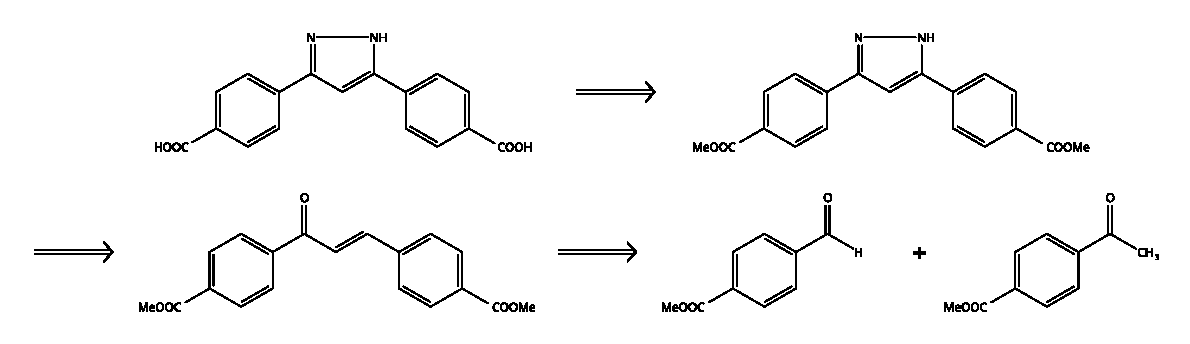
\includegraphics[width=16cm,height=8cm,keepaspectratio]{Structures/pyrazole-retro-alt.eps}
	\caption{Pyrazole Ligand Alternative Retrosynthesis}\label{fig:pyrazole-retro-alt}
\end{figure}

The \(\alpha-\beta\) unsaturated diester intermediate, is asymmetric and carry an olefinic group that should ensure good solubility in less polar organic solvents, allowing to bypass the key problem of solubility encountered with dimethyl 4,4’-malonyldibenzoate.

\subsection{Unsaturaded Diester Formation}\label{sec:alt-pyr-diest}

In order to evaluate the alternative synthetic pathway, with the hope of resolving the series of criticalities encountered, the conditions of formation of the first product reported in the retrosynthesis were evaluated.

\begin{figure}[h!]
	\centering
	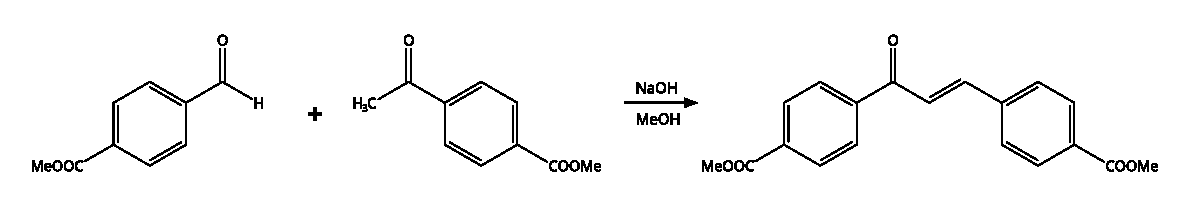
\includegraphics[width=13cm,height=8cm,keepaspectratio]{Structures/unsaturated-synt.eps}
	\caption{Unsaturated Compound Formation}
\end{figure}

The reagents required for the reaction are readily available, and the reaction conditions used follow those classically applied in croton condensation reactions. Some of the variables that can influence the reaction have been analyzed, based on the reagents properties.\\

\subsubsection{Solvent}

As for the solvent MeOH, it seems the easiest choice to avoid transesterification.
Moreover, at the end of the reactions performed, the solvent takes on a yellowish colour that could be associated with the fraction of self-condensation product formed that would then be soluble in MeOH. The condensation product, on the other hand, precipitates quantitatively. This is very useful to avoid any purification steps; any alternative solvent should retain this characteristic.\\
On the basis of the observations, all reactions were carried out in MeOH and the effect of the solvent has not been adequately investigated.

\subsubsection{Reaction Temperature and Reagent Addition}

The ketone could give rise to self-condensation leading to the formation of an unwanted product, reducing the yield and necessitating a purification step. However, the self-condensation reaction is kinetically disadvantageous compared to cross-condensation. For these reasons, a slow addition of the NaOH solution and an ice bath was used.\\
It would also be possible to exploit a slow addition of ketone to a dispersion of NaOH and aldehyde, however this is impractical as the ketone is not soluble in the typical amounts of solvent used and there is a risk of losing some of the reagent in the addition step.\\
Under conditions such as room temperature, 4h reaction time and 1:1 molar ratio of ketone to aldehyde, a yield of 81\% was achieved. This, although satisfactory, can be further optimised.

\subsubsection{Reaction Time}

With regard to the optimal reaction time, some tests were carried out. An increase in reaction time leads to a significant increase in yield without any downside. The results obtained are shown below:


\begin{table}[h!]
	\centering
	\begin{tabular}[b]{cc}
		\toprule
		Time / h & Yield \\
		\midrule
		4        & 81 \% \\
		15       & 89 \% \\
		\bottomrule
	\end{tabular}
	\caption{Reaction time comparison}\label{tab:hydrazine-ratio}
\end{table}

A longer reaction time leads to a significantly higher yield. Since the reaction takes place at room temperature and there are no special requirements in terms of equipment, there is no reason not to exploit this factor to achieve a higher yield.

\subsubsection{Reagent Proportion}

In order to optimise the reaction yield, it was thought that increasing the ratio of aldehyde to ketone might have a positive effect, as it theoretically reduces the possibility of a self-condensation reaction, given the higher aldehyde ratio.
This possibility was tested with a 1.2 molar ratio of aldehyde to ketone, on an overnight reaction time. The results are shown below.

\begin{table}[h!]
	\centering
	\begin{tabular}[b]{cc}
		\toprule
		Aldehyde Molar Ration & Yield \\
		\midrule
		1                     & 89 \% \\
		1.2                   & 94 \% \\
		\bottomrule
	\end{tabular}
	\caption{Molar ratio comparison}\label{tab:hydrazine-ratio}
\end{table}

It is evident that the effect of the slightly higher ratio is positive, but the effects on the reaction yield of even higher molar ratios have not been investigated: it might be interesting to evaluate this in the future.


\subsection{Hydrazine addition to unsaturated precursor}\label{sec:hyd-add-ins}

\begin{figure}[h!]
	\centering
	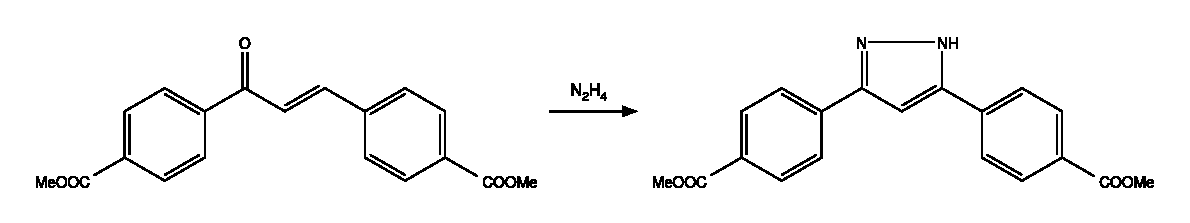
\includegraphics[width=13cm,keepaspectratio]{Structures/pyrazole-form-alternative.eps}
	\caption{Hydrazine reaction with unsaturated compound}
\end{figure}

This step is the crucial one to evaluate the effectiveness of the alternative synthesis, given the difficulties encountered in forming the desired product from diketone.

The reaction mechanism does not differ substantially from that reported for diketone, however several of the difficulties encountered in the previous synthetic pattern, particularly the solubility of the initial compound, should not be encountered in this situation. The mechanism is reported below.

The conditions and results obtained for the formation of the pyrazole ring are evaluated, which include different solvents, catalysts, reaction times and the use of the microwave reactor. The conditions used were chosen from those reported in the literature \cite{leavai_synthesis_2002}, verifying the effectiveness of each procedure and modifying what was reported as needed.

\subsubsection{Acetic Acid}\label{sec:ace-cond}

According to the article in the literature, this synthetic route should be the simplest and most effective one, capable of achieving high reaction yields.\\ The reaction is conducted in acetic acid in the presence of hydrazine, with temperatures and reaction times that may vary depending on the substrate. At the end of the reaction, the product should precipitate spontaneously and the same should be easily recoverable by filtration.

However, on a practical level it was not optimal and the results obtained are discouraging. Neither product nor intermediate formation was observed, which reportedly should have been possible to isolate. No effects were observed even by extending reaction times and raising temperatures. The obtained results are reported below and the detailed experimental information are in the chapter\ \ref{cha:experimental-section}.

\begin{table}[h!]
	\centering
	\begin{tabular}[b]{cccc}
		\toprule
		ID & Temperature [K] & Time [h] & Yield \\
		\midrule
		A  & RT              & 1        & -     \\
		B  & 363             & 3        & -     \\
		C  & 393             & 48       & -     \\
		\bottomrule
	\end{tabular}
	\caption{Acetic acid reaction yields}\label{tab:hydrazine-ratio}
\end{table}

The results obtained did not meet expectations; although the reagent dissolved easily at higher temperatures than in test B, no product was recovered.
In addition, investigation of the composition of the mixture were made difficult by the large amount of acetic acid present. Cooling the mixture succeeded in observing extensive precipitation of what was later identified with difficulty as the initial reagent.

\subsubsection{Methanol with acid and basic catalysis}\label{sec:et-ac-bas}

In addition to the conditions used with acetic acid, which proved to be a failure with this initial reagent, conditions including the use of methanol as a solvent in the presence of acidic and basic catalysts, such as hydrochloric acid and pyridine, are reported in the literature.

In relation to the use of hydrochloric acid as a catalyst the results obtained are poor. The addition of hydrazine to the solution of hydrochloric acid in methanol causes a rather violent reaction, subsequently the initial reactant does not solubilize. In the reaction time no change is observed. No product formation is observed, and the mixture does not develop blue photoluminescence. These reaction conditions were then not further investigated.

Unlike what is found in conditions of acid catalysis, the use of pyridine as a catalyst initially seems to lead to better results.
The initial reactant completely solubilized and the mixture was left to react under reflux.

% TODO: aggiungere condizioni e meccanismo per questa reazione, incluso intermedio ed utilizzo del microonde.
% TODO: sistemare anche quaderno in relazione a quanto visto, gli nmr ora ci sono.

\subsubsection{Ethanol}\label{sec:met-only}

As a result of the difficulties encountered previously, several tests were carried out in ethanol alone, at varying temperatures and reaction times, maintaining the molar ratio costant.

The progress of the reaction was checked at room temperature, in the presence of 3 moles of hydrazine per moles of initial reagent, overnight, under strong stirring. The formation of crystalline product, with blue photolumiscence, was observed. What apparently looked like it might be the desired product, upon coupled NMR analysis such as COSY and NOESY turned out to be the hydrazonic intermediate whose structure is given below.

\begin{figure}[h!]
	\centering
	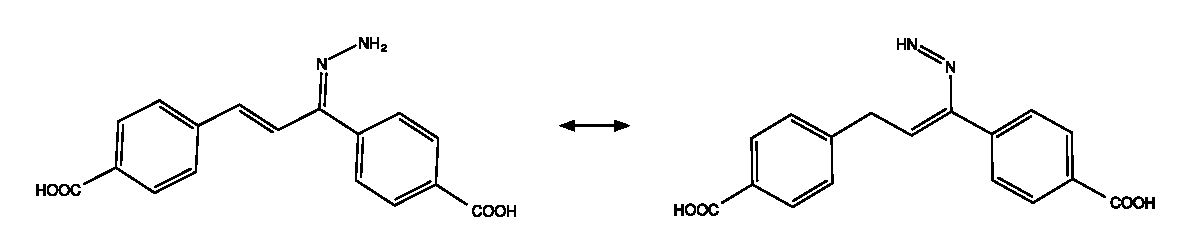
\includegraphics[width=13cm,keepaspectratio]{Structures/idrazone.eps}
	\caption{Intermediate compound structure}
\end{figure}

Indeed, within the literature it was reported that the intermediate could be obtained without proceeding to pyrazole ring closure. By raising the temperature, which should have a positive effect in this case, no change was observed in the product formed despite several hours of reaction. However, the crystallinity of the precipitate formed appears to the eye to be of a higher degree. The structure of the compound identified as an intermediate was again identified using NMR.

\subsubsection{Microwaves}\label{sec:micro}

Microwave reactors have emerged as powerful tools in the field of chemistry \cite{priecel_advantages_2019}, offering numerous advantages over traditional heating methods.

\begin{figure}[h!]
	\centering
	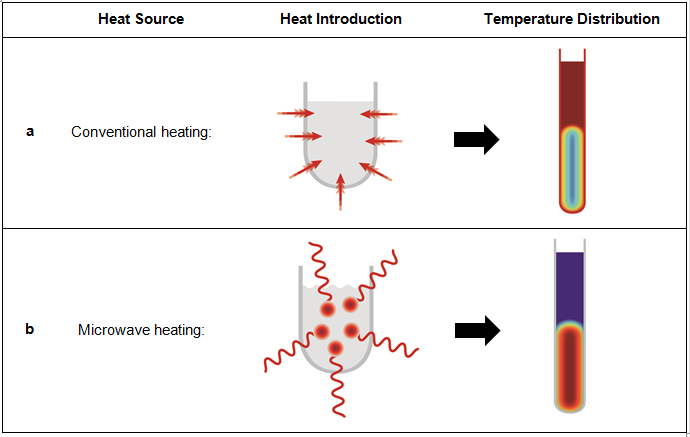
\includegraphics[width=8cm,keepaspectratio]{Images/05_microwave-heat-introduction.jpg}
	\caption{A good representation of the fundamental difference between traditional heating methods and microwaves, where the heat actually comes from the ``inside''.}
\end{figure}

They are able to heat reaction mixtures very quickly, promoting mixing. They also provide granular control of temperature curves and easily allow working at pressures above atmospheric, reaching temperatures above the boiling temperature of the solvent itself at SATP. The amount of solvent used is small, it is not challenging to run reactions with small amounts, and the whole process is energy efficient.

Especially with regard to cyclization reactions and the formation of pyrazolines, several examples are available in the literature \cite{azarifar_microwave-assisted_2003}. The high temperature and pressure make the reactions more selective by providing higher yields; in addition, reaction times are greatly reduced from hours to tens of minutes.

\subsection{Pyrazole Ester Hydrolisis}\label{sec:pyrazole-hydro}

\begin{figure}[h!]
	\centering
	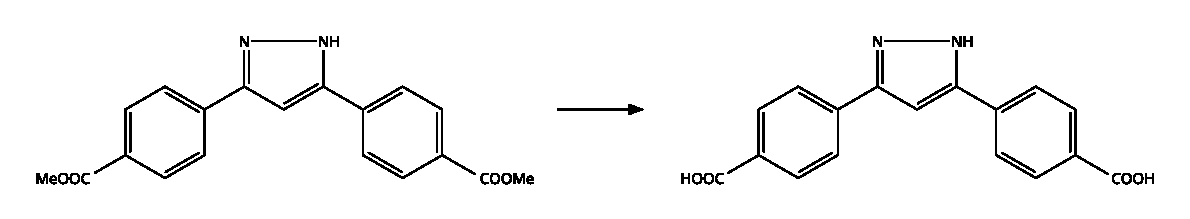
\includegraphics[width=13cm,height=8cm,keepaspectratio]{Structures/pyrazole-hydro.eps}
	\caption{Pyrazole Diester Hydrolisis}\label{fig:pyrazole-form}
\end{figure}

The removal of methyl esters is a standard practice in organic chemistry, and no specific problems were encountered during this step of the synthesis.Two synthetic routes were analyzed.
Initially, removal with LiOH in THF:H$_2$O 1:1 was used, but the yields of the different reactions were not highly reproducible, perhaps because of the precariousness of the different impurities resulting from the different methods of pyrazole synthesis. \\
Instead, removal with NaOH in MeOH:H$_{2}$O 1:1 could give better results, with higher yield and cleaner processing. \\
It is important to note, however, that the results obtained refer to small amounts of reagent, often containing impurities, this due to the large diffculty in obtaining the ester. Thus, this aspect of the synthesis will have to be finalized when the ester synthesis is optimized.

\todo[inline]{mancano rese e risultati ottenuti}


% TODO: rese e risultati ottenuti


\subsection{Conclusion, consideration and further development}\label{sec:conclusioni}

% TODO: aggiungere considerazioni riguardo ai risultati ottenuti. Bene l'aldolica rispetto alla claisen, male la parte di pirazolo, peccato per la one pot. Utilizzo di strada alternativa con coupling.

\newpage\section{Electrochemistry}\label{sec:electrochemistry}

\subsection{Why electrochemistry and cyclic voltammetry?}\label{sec:elect-intro}

Cyclic voltammetry (CV) is a technique used in the analysis of organic and inorganic compounds\ \cite{elgrishi_practical_2018}. It provides information about reduction and oxidation processes of molecular species, the stability, the conversion and storage of energy and several other interesting properties. CV is also invaluable to study electron transfer-initiated chemical reactions, which includes catalysis. CV can be used to estimate the electron affinity and ionization energy of test compounds in a much cheaper and faster way compared to other high vacuum methods. It is important in electrochemistry because it allows to study the electron transfer processes that are at the center of the reactivity of inorganic complexes.
The aforementioned parameters correlate with the energy levels of highest occupied molecular orbital (HOMO) and lowest unoccupied molecular orbital (LUMO).

When cyclic voltammetry (CV) is combined with or ultraviolet-visible and near-infrared (UV-Vis-NIR) spectroscopies, it provides useful information such as electron affinity, ionization potential, band-gap energies, the type of charge carriers, and degradation information\ \cite{pluczyk_using_2018}. Analizing the CV experiment data is possible to determine the band-gap value that can be later evaluted against the one obtained from the spectroscopic UV data.

\subsubsection{Ligands and  Background}
Electrochemistry exploration has been carried out on already studied compounds\ \cite{carlucci_heterometallic_2010}, that have been already synthetized and studied. Structure and synthesis of ligand and monomers  are given below, details of reaction conditions are given in section\ \ref{cha:experimental-section}.

\begin{figure}[h!]
	\centering
	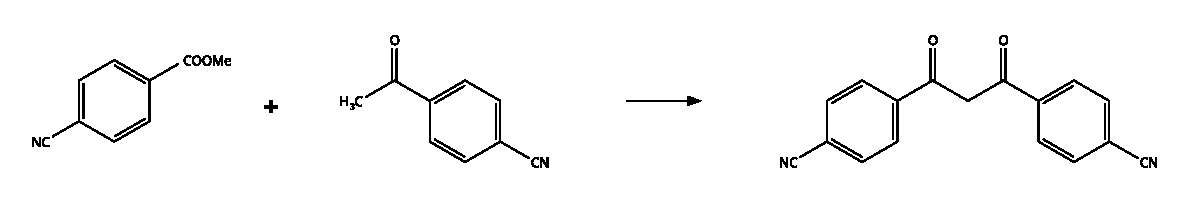
\includegraphics[width=16cm,height=8cm,keepaspectratio]{Structures/dicn-sint.eps}\caption{4‐[3‐(4‐cyanophenyl)‐3‐oxopropanoyl]benzonitrile}
\end{figure}
\todo[inline]{mancano risultati ottenuti}

% TODO: aggiungere risultati ottenuti
% TODO: spiegare meglio la storia del legante e da dove deriva, le sue caratteristiche citando i lavori passati.

\end{document}

%%% Local Variables:
%%% mode: latex
%%% TeX-master: "../Master"
%%% End:


